\documentclass[a4paper,12pt]{article} % This defines the style of your paper

\usepackage[top = 2.5cm, bottom = 2.5cm, left = 2.5cm, right = 2.5cm]{geometry} 

% Unfortunately, LaTeX has a hard time interpreting German Umlaute. The following two lines and packages should help. If it doesn't work for you please let me know.
\usepackage[T1]{fontenc}
\usepackage[utf8]{inputenc}
\usepackage{pifont}
% \usepackage{ctex}
\usepackage{amsthm, amsmath, amssymb, mathrsfs,mathtools}

% Defining a new theorem style without italics
\newtheoremstyle{nonitalic}% name
  {\topsep}% Space above
  {\topsep}% Space below
  {\upshape}% Body font
  {}% Indent amount
  {\bfseries}% Theorem head font
  {.}% Punctuation after theorem head
  {.5em}% Space after theorem head
  {}% Theorem head spec (can be left empty, meaning ‘normal`)
  
\theoremstyle{nonitalic}
% Define new 'solution' environment
\newtheorem{solution}{Solution}

% % Custom counter for the solutions
% \newcounter{solutionctr}
% \renewcommand{\thesolutionctr}{(\alph{solutionctr})}

% % Environment for auto-numbering with custom format
% \newenvironment{autosolution}
%   {\stepcounter{solutionctr}\begin{solution}{\thesolutionctr}}
%   {\end{solution}}


\newtheorem{problem}{Problem}
\usepackage{color}

% The following two packages - multirow and booktabs - are needed to create nice looking tables.
\usepackage{multirow} % Multirow is for tables with multiple rows within one cell.
\usepackage{booktabs} % For even nicer tables.

% As we usually want to include some plots (.pdf files) we need a package for that.
\usepackage{graphicx} 
\usepackage{subfigure}


% The default setting of LaTeX is to indent new paragraphs. This is useful for articles. But not really nice for homework problem sets. The following command sets the indent to 0.
\usepackage{setspace}
\setlength{\parindent}{0in}
\usepackage{longtable}

% Package to place figures where you want them.
\usepackage{float}

% The fancyhdr package let's us create nice headers.
\usepackage{fancyhdr}

\usepackage{fancyvrb}

%Code environment 
\usepackage{listings} % Required for insertion of code
\usepackage{xcolor} % Required for custom colors

% Define colors for code listing
\definecolor{codegreen}{rgb}{0,0.6,0}
\definecolor{codegray}{rgb}{0.5,0.5,0.5}
\definecolor{codepurple}{rgb}{0.58,0,0.82}
\definecolor{backcolour}{rgb}{0.95,0.95,0.92}

% Code listing style named "mystyle"
\lstdefinestyle{mystyle}{
    backgroundcolor=\color{backcolour},   
    commentstyle=\color{codegreen},
    keywordstyle=\color{magenta},
    numberstyle=\tiny\color{codegray},
    stringstyle=\color{codepurple},
    basicstyle=\ttfamily\footnotesize, % Change to serif font
    breakatwhitespace=false,         
    breaklines=true,                 
    captionpos=b,                    
    keepspaces=true,                 
    numbers=left,                    
    numbersep=5pt,                  
    showspaces=false,                
    showstringspaces=false,
    showtabs=false,                  
    tabsize=2
}

\lstset{style=mystyle}

% tikz
\usepackage{tikz}
\usepackage{tikz-cd}
\usepackage{tikzsymbols} % for symbols such as smiley
\usetikzlibrary{intersections, angles, quotes, calc, positioning}
\usetikzlibrary{arrows.meta}
\usepackage{pgfplots}
\pgfplotsset{compat=1.13}


\tikzset{
    force/.style={thick, {Circle[length=2pt]}-stealth, shorten <=-1pt}
}


% theorems
\usepackage{thmtools}
\usepackage[framemethod=TikZ]{mdframed}

%%%%%%%%%%%%%%%%%%%%%%%%%%%%%%%%%%%%%%%%%%%%%%%%
% 3. Header (and Footer)
%%%%%%%%%%%%%%%%%%%%%%%%%%%%%%%%%%%%%%%%%%%%%%%%

% To make our document nice we want a header and number the pages in the footer.

\pagestyle{fancy} % With this command we can customize the header style.

\fancyhf{} % This makes sure we do not have other information in our header or footer.

\lhead{\footnotesize EI135 International Trade I}% \lhead puts text in the top left corner. \footnotesize sets our font to a smaller size.

%\rhead works just like \lhead (you can also use \chead)
\rhead{\footnotesize Jingle Fu} %<---- Fill in your lastnames.

% Similar commands work for the footer (\lfoot, \cfoot and \rfoot).
% We want to put our page number in the center.
\cfoot{\footnotesize \thepage}
\IfFileExists{upquote.sty}{\usepackage{upquote}}{}
\begin{document}


\thispagestyle{empty} % This command disables the header on the first page. 

\begin{tabular}{p{15.5cm}} % This is a simple tabular environment to align your text nicely 
{\large \bf EI135 International Trade I} \\
The Graduate Institute, Spring 2025\\
\hline % \hline produces horizontal lines.
\\
\end{tabular} % Our tabular environment ends here.

\vspace*{0.3cm} % Now we want to add some vertical space in between the line and our title.

\begin{center} % Everything within the center environment is centered.
	{\Large \bf PS1 Solutions} % <---- Don't forget to put in the right number
	\vspace{2mm}
	
        % YOUR NAMES GO HERE
	{\bf Jingle Fu \& Yingjie Zhang} % <---- Fill in your names here!
		
\end{center}  

\vspace{0.4cm}
\setstretch{1.2}

\begin{solution}[Gains from Trade]
    \

    Assuming the consumption bundle of Australia(A) before trading with China is $\mathbf{c_1}$ and after is $\mathbf{c_2}$.

    Before China's involvement, according to the Weak Axiom of Revealed Preference, we have $\mathbf{p_1} \mathbf{c_1} \leq \mathbf{p_1} \mathbf{c_2}.$

    After China's entering, we have $\mathbf{p_2} \mathbf{c_2} \leq \mathbf{p_2} \mathbf{c_1}.$
\end{solution}

\begin{solution}[Ricardian Trade and Technological Progress]
    \

    \begin{enumerate}
        \item[1.] For absolute advantage, we compare unit labor productivity directly:
            \begin{itemize}
                \item Clothing
                \begin{itemize}
                \item Home: produces $z$ unit per hour.
                \item Foreign: produces 1 unit per hour.
                \end{itemize}
                Home has an absolute advantage in clothing if $z>1$; otherwise, Foreign does.
                \item Food
                \begin{itemize}
                \item Home: produces $z$ unit per hour.
                \item Foreign: produces 4 unit per hour.
                \end{itemize}
                Home has an absolute advantage in food if $z>4$; otherwise, Foreign does.
            \end{itemize}
            Thus, comparing the absolute advantage, we have the following table:
            \begin{table}[H]
                \centering
                \begin{tabular}{c|c|c}
                \toprule
                & Clothing & Food \\
                \midrule
                $z>4$ & Home & Home \\
                $1<z<4$ & Home & Foreign \\
                $z<1$ & Foreign & Foreign \\
                \bottomrule
                \end{tabular}
            \end{table}
        \item[2.] For comparative advantage, we compare the opportunity cost of producing one unit of one good in terms of the other good:
            \begin{itemize}
                \item Home: The opportunity cost of 1 unit of Clothing over 1 unit of Food is: $\frac{a_C}{a_F} = 1$.
                \item Foreign: The opportunity cost of 1 unit of Clothing over 1 unit of Food is: $\frac{a_C^*}{a_F^*} = 4$.
            \end{itemize}
            Thus, Home has a comparative advantage in Clothing, and Foreign has a comparative advantage in Food, regardless of $z$.
        \item[3.] If $z=2$, the relative price of Clothing is $P = \frac{P_C}{P_F} = \frac{a_C}{a_F} = 1$, $P^* = \frac{a_C^*}{a_F^*} = 4$.\\
            $Q_C = \frac{L}{a_C} = 2000 = Q_F$, $Q_C^* = \frac{L^*}{a_C^*} = 1000$, $Q_F^* = \frac{L^*}{a_F^*} = 4000.$
            \begin{enumerate}
                \item[(a)] Draw the world relative supply of clothing.
                    \begin{itemize}
                        \item When $P<1$, both Home and Foreign produce only Food, giving $R = \frac{Q_C + Q_C^*}{Q_F + Q_F^*} = 0$;
                        \item When $P=1$, Home can vary production between $(\text{Clothing}, \text{Food}) = \Bigl[(2000, 0), (0,2000)\Bigr]$ and Foreign produces only Food, giving $R \in [0, 0.5]$;
                        \item When $1<P<4$, Home produces only Clothing and Foreign produces only Food, giving $R = 0.5$;
                        \item When $P=4$, Home produces only Clothing and Foreign can vary production between $(\text{Clothing}, \text{Food}) = \Bigl[(0,4000), (1000, 0)\Bigr]$, giving $R \in [0.5, \infty)$;
                        \item When $P>4$, both Home and Foreign produce only Clothing, giving $R = \infty$.
                    \end{itemize}
                    \begin{center}
                        \begin{tikzpicture}[scale=1.2]
                            % Axes
                            \draw[->] (0,0) -- (5,0) node[right] {$R = \frac{Q_C}{Q_F}$};
                            \draw[->] (0,0) -- (0,5) node[above] {$P = \frac{P_C}{P_F}$};
                            
                            % Critical price lines
                            \draw[dashed] (0,1) -- (5,1) node[left] at (0,1) {$1 = \frac{a_C}{a_F}$};
                            \draw[dashed] (0,4) -- (5,4) node[left] at (0,4) {$4 = \frac{a_C^*}{a_F^*}$};
                                
                            % World Relative Supply curve
                            \draw[thick, blue] (0,0) -- (0,1) -- (0.5,1) -- (0.5,4) -- (5,4);
                            % -- (4.5,5)
                            % Points for clarification
                            \fill[blue] (0,0) circle (2pt);
                            \fill[blue] (0,1) circle (2pt);
                            \fill[blue] (0.5,1) circle (2pt);
                            \fill[blue] (0.5,4) circle (2pt);
                            % \fill[blue] (4.5,4) circle (2pt);
                            % \fill[blue] (4.5,5) circle (2pt);               
                            % % Region labels
                            % \node[blue, scale=0.8, align=left] at (0.3,0.5) {Both produce Food};
                            % \node[blue, scale=0.8, align=center] at (0.25,1.5) {Home varies\\Foreign: Food};
                            % \node[blue, scale=0.8, align=center] at (0.7,2.5) {Home: Clothing\\Foreign: Food};
                            % \node[blue, scale=0.8, align=center] at (2.5,4.5) {Home: Clothing\\Foreign varies};
                            % \node[blue, scale=0.8, align=right] at (4,4.7) {Both produce Clothing};
                            
                            % X-axis markers
                            \node[below] at (0,0) {$0$};
                            \node[below] at (0.5,0) {$0.5$};
                            \node[below] at (4.5,0) {$\infty$};
                        \end{tikzpicture}
                    \end{center}
                \item[(b)] Under the Cobb-Douglas utility function $U(C, F) = CF$, we can tell that consumers will spend the same expenditure on both goods.
                So, worldwide, $P_C Q_C = P_F Q_F$, which gives $\frac{P_C}{P_F} = \frac{Q_F}{Q_C} = \frac{1}{R} = 2.$
                
                \begin{center}
                    \begin{tikzpicture}[scale=1.2]
                        % Axes
                        \draw[->] (0,0) -- (5,0) node[right] {$R = \frac{Q_C}{Q_F}$};
                            \draw[->] (0,0) -- (0,5) node[above] {$P = \frac{P_C}{P_F}$};
                            
                            % Critical price lines
                            \draw[dashed] (0,1) -- (5,1) node[left] at (0,1) {$1 = \frac{a_C}{a_F}$};
                            \draw[dashed] (0,4) -- (5,4) node[left] at (0,4) {$4 = \frac{a_C^*}{a_F^*}$};
                                
                            % World Relative Supply curve
                            \draw[thick, blue] (0,0) -- (0,1) -- (0.5,1) -- (0.5,4) -- (5,4);

                        % New equilibrium points (adjusted)
                        \node[circle, fill, red, inner sep=1.5pt, label={[blue]above right:A}] at (0.5,2) {};
                        
                        % Indifference curves (parallel)
                        % Curve A passing through (0.6,0.8)
                        \draw[red, thick] plot[domain=0.3:2.5, samples=100] (\x, {1/\x});

                        % X-axis markers
                        \node[below] at (0,0) {$0$};
                        \node[below] at (0.5,0) {$0.5$};
                        \node[below] at (4.5,0) {$\infty$};
                    \end{tikzpicture}
                \end{center}

                \item[(c)] In Home, a worker produces $z=2$ units of Clothing per hour, hence the value of one hour's output is: $w = 2 P_C$;
                While in foreign, a worker produces 4 units of Food per hour, having a value of $p^* = 4 P_F$.
                Given that $\frac{P_C}{P_F} = 2$, we know it that $\frac{w}{w^*} = 1.$
            \end{enumerate}
        \item[4.] As analyzed before, the change of $z$ won't affect the world relative price.
        We assume that after the change both countries remain completely specialized in their comparative-advantage goods.
            \begin{enumerate}
                \item[(a)] Home produces $1000z$ units of Clothing, and Foreign produces 4000 unnits of food.
                The world relative supply of Clothing is $R = \frac{1000z}{4000} = \frac{z}{4}$.

                For Home, a worker's nominal income is $w = z P_C$, and for Foreign, $w^* = 4 P_F$.

                Our Cobb-Douglas utility with equal share tells us that $P = \frac{P_C}{P_F} = \frac{Q_F}{Q_C} = \frac{1}{R}$, thus $P = \frac{4}{z}$.

                Thus the free-trade relative price is $\frac{P_C}{P_F} = \frac{4}{z}$, the wage ratio is:
                \[\frac{w}{w^*} = \frac{z P_C}{4 P_F} = 1. \]
                \item[(b)] If $z$ increases, the relative price $P = \frac{4}{z}$ decreases, since the 
            \end{enumerate}
    \end{enumerate}
\end{solution}

\begin{solution}[Two-by-Two-by-Two with Fixed Coefficients]
    \
    
    \begin{enumerate}
        \item[1.] 
        \begin{itemize}
            \item \textbf{Relative Factor Abundance:} $RFA_A = \frac{K_A}{L_A} = \frac{420}{460} \approx 1.095$, $RFA_G = \frac{K_G}{L_G} = \frac{900}{600} = 1.5$. Thus Germany is relatively capital abundant and Austria is relatively labor abundant.
            \item \textbf{Relative Factor Intensity of Goods:} $RFIG_B = \frac{a_{KB}}{a_{LB}} = 3$, $RFIG_S = \frac{a_{KS}}{a_{LS}} = 0.5$. Thus Buns are capital intensive, while Sausages are labor intensive.
            \item \textbf{Comparative Advantage:} By the Heckscher-Ohlin theorem, the relatively capital-abundant country, Germany, 
            will have a comparative advantage in the capital-intensive good, Buns, 
            and the relatively labor-abundant country, Austria, in the labor-intensive good, Sausages.
            \item \textbf{Autarkic Relative Price:} In autarky, each country's relative price reflects its ``shadow'' cost. Because factor prices adjust differently in each country (with the excess factor receiving a zero ``price''), we expect:
                \begin{itemize}
                    \item Austria: As labor is in excess, the wage is set to 0, hence $P_A = \frac{P_{BA}}{P_{SA}} = \frac{a_{KB}}{a_{KS}} = 3$;
                    \item Germany: As capital is in excess, the rental rate is set to 0, hence $P_G = \frac{P_{BG}}{P_{SG}} = \frac{a_{LB}}{a_{LS}} = \frac{1}{2}$.
                \end{itemize}
                Thus, the autarkic price of Buns is higher in Austria than in Germany. Under trade we expect Germany to export Buns and Austria to export Sausages.
            \item \textbf{Free Trade:} Under trade we expect Germany to export Buns and Austria to export Sausages.
        \end{itemize}

        \item[2.] We separate the two countries' production functions and factor endowments: $B = Q_{BA} + Q_{BG}$, $S = Q_{SA} + Q_{SG}$.
        \begin{enumerate}
            \item[(a)] For Austria, the full employment conditions are:
            \begin{itemize}
                \item \textbf{Labor:} 
                \[ L_A = a_{LB} Q_{BA} + a_{LS} Q_{SA} \Rightarrow Q_{BA} + 2 Q_{SA} = 420\]
                \item \textbf{Capital:}
                \[ K_A = a_{KB} Q_{BA} + a_{KS} Q_{SA} \Rightarrow 3 Q_{BA} + Q_{SA} = 460\]
            \end{itemize}
            Both constraints hold with equality, we can have: $(Q_{BA}, Q_{SA}) = (100, 160).$
            \begin{center}
                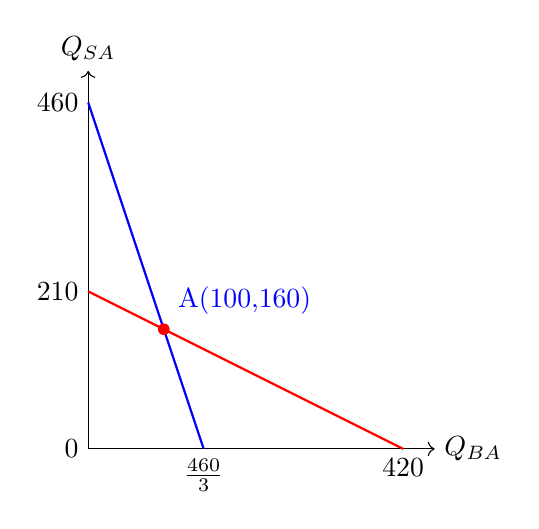
\begin{tikzpicture}[scale=0.8]
                    % Axes
                    \draw[->] (0,0) -- (5.5,0) node[right] {$Q_{BA}$};
                    \draw[->] (0,0) -- (0,6) node[above] {$Q_{SA}$};
                    
                    % Indifference curves
                    \draw[red, thick] plot[domain=0:5, samples=100] (\x, {5/2 - \x/2});
                    \draw[blue, thick] plot[domain=0:1.8333, samples=100] (\x, {5.5 - 3*\x});
                    
                    % Equilibrium point
                    \node[circle, fill, red, inner sep=1.5pt, label={[blue]above right:A(100,160)}] at (1.2,1.9) {};
                    
                    % X-axis markers
                    \node[below] at (1.8333,0) {$\frac{460}{3}$};
                    \node[below] at (5,0) {$420$};
                    % Y-axis markers
                    \node[left] at (0,0) {$0$};
                    \node[left] at (0,2.5) {$210$};
                    \node[left] at (0,5.5) {$460$};
                \end{tikzpicture}
            \end{center}
        
            \item[(b)] For Germany, the full employment conditions are:
            \begin{itemize}
                \item \textbf{Labor:} 
                \[ L_G = a_{LB} Q_{BG} + a_{LS} Q_{SG} \Rightarrow Q_{BG} + 2 Q_{SG} = 600\]
                \item \textbf{Capital:}
                \[ K_G = a_{KB} Q_{BG} + a_{KS} Q_{SG} \Rightarrow 3 Q_{BG} + Q_{SG} = 900\]
            \end{itemize}
            Solve the equations, we have: $(Q_{BG}, Q_{SG}) = (240, 180).$
            \begin{center}
                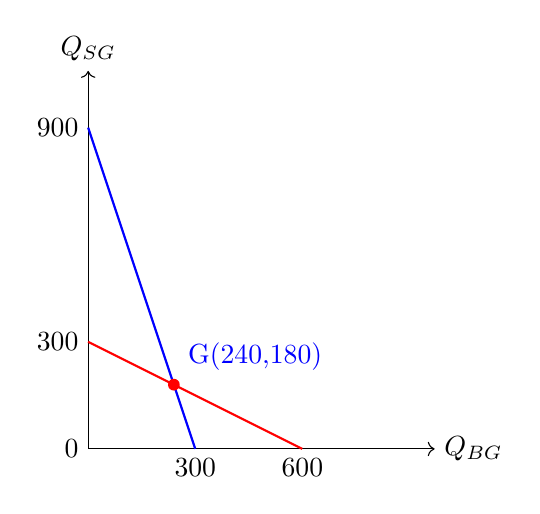
\begin{tikzpicture}[scale=0.8]
                    % Axes
                    \draw[->] (0,0) -- (5.5,0) node[right] {$Q_{BG}$};
                    \draw[->] (0,0) -- (0,6) node[above] {$Q_{SG}$};
                    
                    % Indifference curves
                    \draw[red, thick] plot[domain=0:3.4, samples=100] (\x, {3.4/2 - \x/2});
                    \draw[blue, thick] plot[domain=0:1.7, samples=100] (\x, {5.1 - 3*\x});
                    
                    % Equilibrium point
                    \node[circle, fill, red, inner sep=1.5pt, label={[blue]above right:G(240,180)}] at (1.36,1.02) {};
                    
                    % X-axis markers
                    \node[below] at (1.7,0) {$300$};
                    \node[below] at (3.4,0) {$600$};
                    % Y-axis markers
                    \node[left] at (0,0) {$0$};
                    \node[left] at (0,1.7) {$300$};
                    \node[left] at (0,5.1) {$900$};
                \end{tikzpicture}
            \end{center}
        \end{enumerate}

        \item[3.] Consumers have Leontief preferences (they want to consume 1 Bun and 1 Sausage per hotdog). Because the consumption ratio is fixed at 1, autarkic equilibrium production must satisfy $B=S$.
            \begin{enumerate}
                \item[(a)] We first find the ebalanced production point in both countries:
                    \begin{itemize}
                        \item Austria: 
                            \begin{align*}
                                \text{Labor: } & B + 2B \leq 420 \\
                                \text{Capital: } & 3B + B \leq 460
                            \end{align*}
                            The binding constraint is capital, so the maximum balanced production in Austria is $B = S = 115$.
                        \item Germany:
                            \begin{align*}
                                \text{Labor: } & B + 2B \leq 600 \\
                                \text{Capital: } & 3B + B \leq 900
                            \end{align*}
                            The binding constraint is labor, so the maximum balanced production in Germany is $B = S = 200$.
                    \end{itemize}
                    The autarkic relative price is set by the zero-profit conditions.

                    For Austria, as balanced production $(115, 115)$ lies in the interior of the production possibilities frontier, labor is in excess. (Thus $W = 0$, and prices are determined solely by the rental rate $R$.)

                    In Germany, capital is in excess, so $R = 0$.

                    The zero-profit conditions then are:
                        \begin{align*}
                            P_{BA} &= W + 3R = 3R \\
                            P_{SA} &= 2W + R = R \\
                            P_{BG} &= W \\
                            P_{SG} &= 2W
                        \end{align*}
                    These relative prices are in line with our prediction from part (1).

                \item[(b)] In Austria, labor is in excess, hence $W=0$.  Total national income is $R\cdot K_A = 460R.$
                Each hotdog costs $P_{BA} + P_{SA} = 4R$, so each owner of a unit of capital can buy $\frac{R}{4R} = \frac{1}{4}$ hotdogs.
                
                In Germany, capital is in excess, so $R = 0$. Total income is $W \cdot L_G = 600W$.
                Each hotdog costs $P_{BG} + P_{SG} = 3W$, so each worker can buy $\frac{W}{3W} = \frac{1}{3}$ hotdogs.
            \end{enumerate}
        
            \item[4.]
                \begin{enumerate}
                    \item[(a)] As $P = \frac{P_B}{P_S} = 2 \in [P_G, P_A]$, Germany produces only buns and Austria produces only sausages.
                \end{enumerate}
    \end{enumerate}
\end{solution}

\begin{solution}[Two-by-Two-by-Two]
    \

    \begin{enumerate}
        \item[1.] Each country produces two goods using:
            \begin{itemize}
                \item \textbf{Good 1:} $x_1 = L_1$, only labor used,
                \item \textbf{Good 2:} $x_2 = K_2$, only capital used.
            \end{itemize}
            In any competitive equilibrium, the price of each good equals unit cost: $p_1 = w_J$, $p_2 = r_J$.
            As the household's utility is an 'equal-exponent' cobb-Douglas function, the expenditure on each good is the same, giving $p_1 c_1 = p_2 c_2$.
            Thus $\frac{p_1}{p_2} = \frac{c_2}{c_1}$. In autarky equilibrium, comsumptions equals output, thus
            $c_{1J} = x_{1J} =L_J$ and $c_{2J} = x_{2J} = K_J$. With $Y_J = w_J L_J + r_J K_J$, we know that $w_J L_J = r_J K_J.$

            Thus in autarky, the relative price of Good 1 is $p_1/p_2 = w_J/r_J = K_J/L_J$.

        \item[2.] Now if two countries integrate, then both countries have the same wage and rental rate: $p_1 = w$ and $p_2 = r$.
        Households, with the same preferences, spend half their income on each good, where income is $Y = w(L_H + L_F) + r(K_H + K_F)$.
        Based on similar analysis, we know that $\frac{w}{r} = \frac{K_H + K_F}{L_H + L_F} = 1.$ Determined by world endowments and preferences.

        \item[3.] Now suppose that goods trade is free but factors are immobile internationally. 
        In that case each country`s factor market outcome remains as in autarky, so we have:
        \begin{itemize}
            \item \textbf{Home:} $\frac{p_{1H}}{p_{2H}} = \frac{w_H}{r_H} = \frac{K_H}{L_H} = 3$,
            \item \textbf{Foreign:} $\frac{p_{1F}}{p_{2F}} = \frac{w_F}{r_F} = \frac{K_F}{L_F} = \frac{1}{3}$.
        \end{itemize}
        In this trade equilibrium, factor price equalization (FPE) does not occur because factor markets remain separated.
        Each country`s wages and rental rates continue to be determined by its own factor endowment.

        \item[4.] Because factor prices in a competitive industry must equal the unit cost of production, the zero-profit conditions now read:
        In country H, if producing good 1, $p_1 = \frac{w_H}{9}$; if producing good 2, $p_2 = w_F$. As bufore, for good 2 $p_2 = r$ holds in either country.
        
        FPE requires identical production technologies (or, more precisely, identical “unit cost functions”) 
        so that the goods-market equilibrium forces the same factor prices everywhere. Here, even if the same world goods prices prevail, 
        the “effective” unit cost for good 1 differs across countries.

        Thus, even under free goods trade the domestic factor prices in will remain different. 
        In other words, the equilibrium will not exhibit factor price equalization.

        \item[5.] W.l.o.g, we normalize $p_1 =1$ and $p_2 = P$.
            \begin{itemize}
                \item Country H: When producing good 1, $1 = \frac{w_H}{9} \Rightarrow w_H = 9$.
                    When producing good 2, $P = r_H$.
                \item Country F: When producing good 1, $1 = w_F$.
                    When producing good 2, $P = r_F$.
            \end{itemize}
            Notice that for good 1 the effective cost in $H$ is: $\frac{w_H}{9} = 1$, and in $F$ is $w_F = 1$.
            Thus, both countries are “equally efficient” in producing good 1 in terms of cost. 
        \item[6.]
        \item[7.]    
    \end{enumerate}
\end{solution}

\begin{solution}[Gravity with Multilateral Resistance]
    \

    Let the income of country $j$ denoted by $Y_j$, and the price of a good from country $i$ in country $j$ be $p_{ij}$.
    For consumers, their UMP is:
    \begin{align*}
        \max_{x_{kj}} & \Bigl[ \sum_k \alpha_{kj}^{\frac{1}{\sigma}} x_{kj}^{\frac{\sigma-1}{\sigma}}\Bigr]^{\frac{\sigma}{\sigma-1}} \\
        \text{s.t. } & \sum_k x_{kj} p_{kj} \leq Y_j
    \end{align*}
    Define the Lagrangian:
    \begin{gather*}
        \mathcal{L} = \Bigl[ \sum_k \alpha_{kj}^{\frac{1}{\sigma}} x_{kj}^{\frac{\sigma-1}{\sigma}}\Bigr]^{\frac{\sigma}{\sigma-1}} - \lambda \Bigl( \sum_k x_{kj} p_{kj} - Y_j \Bigr)
    \end{gather*}
    The FOCs are:
    \begin{align}
        \frac{\partial \mathcal{L}}{\partial x_{kj}} &= \Bigl[ \sum_k \alpha_{kj}^{\frac{1}{\sigma}} x_{kj}^{\frac{\sigma-1}{\sigma}}\Bigr]^{\frac{1}{\sigma-1}} \alpha_{kj}^{\frac{1}{\sigma}} x_{kj}^{-\frac{1}{\sigma}} - \lambda p_{kj} = 0 \\
        \frac{\partial \mathcal{L}}{\partial \lambda} &= \sum_k x_{kj} p_{kj} - Y_j = 0
    \end{align}
    From (1), we know that for two countries $k$ and $k^{\prime}$, we have:
    \[
    \frac{p_{kj}}{p_{k^{\prime} j}} = \frac{\alpha_{kj}^{\frac{1}{\sigma}} x_{kj}^{-\frac{1}{\sigma}}}{\alpha_{k^{\prime} j}^{\frac{1}{\sigma}} x_{k^{\prime} j}^{-\frac{1}{\sigma}}} \Leftrightarrow \frac{\alpha_{kj}}{\alpha_{k^{\prime} j}} = \frac{p_{kj}^{\sigma}}{p_{k^{\prime} j}^{\sigma}} \frac{x_{kj}}{x_{k^{\prime} j}}
    \]
    Rearranging and multiplying both sides by $p_{k^{\prime} j}$ yields:
    \[
    x_{k^{\prime} j} p_{k^{\prime} j} = \frac{1}{\alpha_{kj}} x_{kj} p_{kj}^{\sigma} \alpha_{k^{\prime} j} p_{k^{\prime} j}^{1-\sigma}
    \]
    Summing for all countries gives:
    \begin{gather}
        \sum_{k^{\prime}} x_{k^{\prime} j} p_{k^{\prime} j} = \frac{1}{\alpha_{kj}} x_{kj} p_{kj}^{\sigma} \sum_{k^{\prime}} \alpha_{k^{\prime} j} p_{k^{\prime} j}^{1-\sigma} \Leftrightarrow Y_j = \frac{1}{\alpha_{kj}} x_{kj} p_{kj}^{\sigma} P_j^{1-\sigma} 
    \end{gather}
    where $P_j = \Bigl[ \sum_k \alpha_{kj} p_{kj}^{1-\sigma} \Bigr]^{\frac{1}{1-\sigma}}$ is the Dixit-Stiglitz price index.

    Rearrange (3) gives the CES demand function:
    \begin{gather}
        x_{kj} = \alpha_{kj} p_{kj}^{-\sigma} Y_j P_j^{\sigma-1}
    \end{gather}
    Noting that the value of total trade is simply equal to the price times quantity, which gives $X_{kj} = p_{kj} x_{kj}$, we have:
    \begin{gather}
        X_{kj} = \alpha_{kj} p_{kj}^{1-\sigma} Y_j P_j^{\sigma-1}
    \end{gather}

    As we suppose that the market for each country/good is perfectly competitive, the price of a good is simply the marginal cost.
    Let $w_i$ be the wage of a worker in country $i$.

    Because we assume that one unit of labor produces one unit of the local output,
    the wage in country $i$ is simply the price of the good produced in country $i$: $p_i = w_i$.

    So, the price of $j$ consuming 1 unit of country $i$'s good is:
    \begin{gather}
        p_{ij} = \tau_{ij} w_i \Rightarrow \tau_{ij} = \frac{p_{ij}}{p_i}.
    \end{gather}
    \begin{enumerate}
        \item[1.] Let $\lambda_{ij}$ be the share of total spending in country $j$ that is devoted to goods imported
        from country $i$. Implementing (5), (6) and the price index, We have:
        \begin{align*}
            \lambda_{ij} &= \frac{X_{ij}}{Y_j} = \alpha_{ij} p_{ij}^{1-\sigma} P_j^{\sigma-1} \\
            &= \alpha_{ij} \Bigl( \tau_{ij} w_i \Bigr)^{1-\sigma} \Bigl[ \sum_k \alpha_{kj} \Bigl( \tau_{kj} w_k \Bigr)^{1-\sigma} \Bigr]^{\sigma-1} \\
            &= \frac{\alpha_{ij} \tau_{ij}^{1-\sigma} w_i^{1-\sigma}}{\sum_k \alpha_{kj} \Bigl( \tau_{kj} w_k \Bigr)^{1-\sigma}} \tag{*}
        \end{align*}

        \item[2.] As market clearing requires income is equal to payments to, the $Y$ we previously defined is the same as the $X_i$(defined as GDP in country $i$).
        
        Income in a country is also equal to its total sales:
        \begin{gather*}
            X_i = \sum_j X_{ij} = \sum_j \alpha_{ij} \tau_{ij}^{1-\sigma} w_i^{1-\sigma} X_j P_j^{\sigma-1} \\
            \Rightarrow w_i^{1-\sigma} = X_i / \sum_j \alpha_{ij} \tau_{ij}^{1-\sigma} X_j P_j^{\sigma-1}
        \end{gather*}
        Replace this equation back into (5), we have:
        \begin{align*}
            X_{ij} &= \alpha_{ij} \tau_{ij}^{1-\sigma} w_i^{1-\sigma} X_j P_j^{\sigma-1} \\
            &= \alpha_{ij} \tau_{ij}^{1-\sigma} \frac{X_i}{\sum_k \alpha_{ik} \tau_{ik}^{1-\sigma} X_k P_k^{\sigma-1}} X_j P_j^{\sigma-1} \\
            &= X_i X_j \Bigl( \frac{\tau_{ij}}{P_j} \Bigr)^{1-\sigma} \frac{\alpha_{ij}}{\sum_k \alpha_{ik} \Bigl( \frac{\tau_{ik}}{P_k} \Bigr)^{1-\sigma} X_k} \tag{**}
        \end{align*}
        
        \item[3.] Under CES preferences, utility of the representative agent is the real wage. Thus in our notation, we have: $X_j = U_j P_j$.
        The per capita welfare $W_i$ can be written as:
        \begin{gather}
            W_j = \frac{U_j}{L_j} = \frac{X_j}{P_j L_j} = \frac{w_j L_j}{P_j L_j} = \frac{w_j}{P_j}
        \end{gather}
        We assume that $\tau_{jj} = 1$, and by choosing $i=j$, (*) implies:
        \[
        \lambda_{jj} = \alpha_{jj} w_j^{1-\sigma} P_j^{\sigma-1} \Rightarrow P_j = \Bigl( \lambda_{jj} \alpha_{jj}^{-1} w_j^{\sigma-1} \Bigr)^{\frac{1}{\sigma-1}} = \lambda_{jj}^{\frac{1}{\sigma-1}} \alpha_{jj}^{-\frac{1}{\sigma-1}} w_j
        \]
        Replacing this equation into (7), we have:
        \[
        W_j = \frac{w_j}{\lambda_{jj}^{\frac{1}{\sigma-1}} \alpha_{jj}^{-\frac{1}{\sigma-1}} w_j} = \lambda_{jj}^{-\frac{1}{\sigma-1}} \alpha_{jj}^{\frac{1}{\sigma-1}} \tag{***}
        \]
    \end{enumerate}
\end{solution}

\end{document}